\documentclass{article}
\usepackage{geometry} % Required for customizing margins
\geometry{margin=1in} % Sets 1-inch margins on all sides
\usepackage{graphicx}
\usepackage{tikz}
\usetikzlibrary{graphs,graphs.standard}

\begin{document}
\title{CSCE 350 Section 001: Assignment \#5}
\author{Jacob C. Vaught}
\date{Oct 31. 2023}
\maketitle
\section*{Problem \#1}

Given the colored graph in Figure \ref{fig:graph}:

\begin{itemize}
    \item Find the BFS traversal starting at vertex `a'.
    \item Construct the corresponding BFS forest.
    \item List the number of tree edges and identify other types of edges.
\end{itemize}
\begin{figure}[h]
\centering
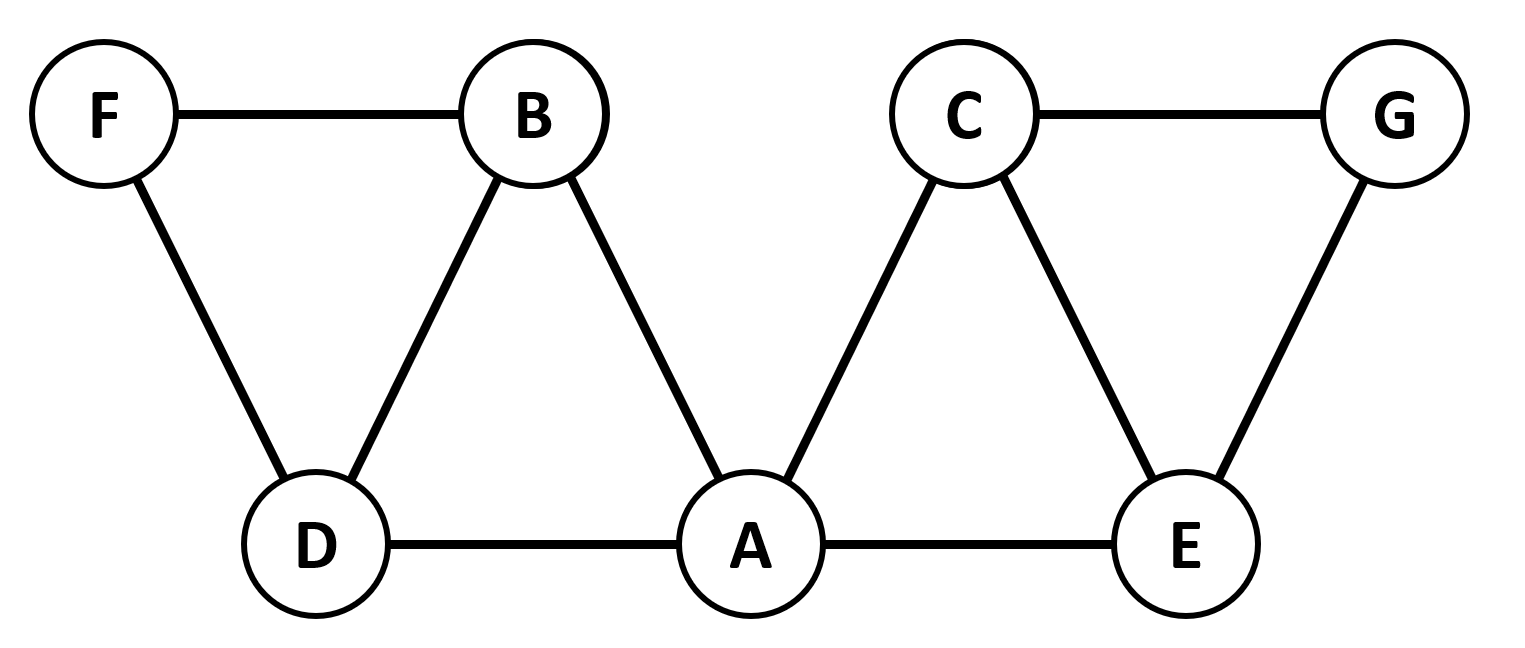
\includegraphics[width=0.7\textwidth]{P1.png}
\caption{Given graph for BFS traversal.}
\label{fig:graph}
\end{figure}

\section*{Solution}

Solving for the Traversal, starting at vertex 'a':

\begin{enumerate}
    \item 
    \begin{minipage}[t]{0.7\textwidth}
    Start at `a':
    \end{minipage}%
    \begin{minipage}[t]{0.3\textwidth}
    BFS order: \(a\)
    \end{minipage}

    \item 
    \begin{minipage}[t]{0.7\textwidth}
    Neighbors of `a': \(b, c, d, e\). Add in alphabetical order:
    \end{minipage}%
    \begin{minipage}[t]{0.3\textwidth}
    BFS order: \(a, b, c, d, e\)
    \end{minipage}

    \item 
    \begin{minipage}[t]{0.7\textwidth}
    Neighbors of `b': \(a, f\). `a' is visited, so add `f':
    \end{minipage}%
    \begin{minipage}[t]{0.3\textwidth}
    BFS order: \(a, b, c, d, e, f\)
    \end{minipage}

    \item 
    \begin{minipage}[t]{0.7\textwidth}
    Neighbors of `c': \(a, e, g\). `a' and `e' are visited, so add `g':
    \end{minipage}%
    \begin{minipage}[t]{0.3\textwidth}
    BFS order: \(a, b, c, d, e, f, g\)
    \end{minipage}

    \item 
    \begin{minipage}[t]{0.7\textwidth}
    Neighbors of `d', `e', `f', and `g' are either `a' or already visited nodes.
    \end{minipage}
\end{enumerate}
Corrected BFS traversal order: \(a, b, c, d, e, f, g\)
\newpage
\noindent Figure \ref{fig:graphsol} shows the process to solve the problem.
Graph with Traversals: Green edges show the primary path, yellow indicates the secondary, and purple marks cross edges (no ancestor-descendant relation).
\begin{figure}[h]
\centering
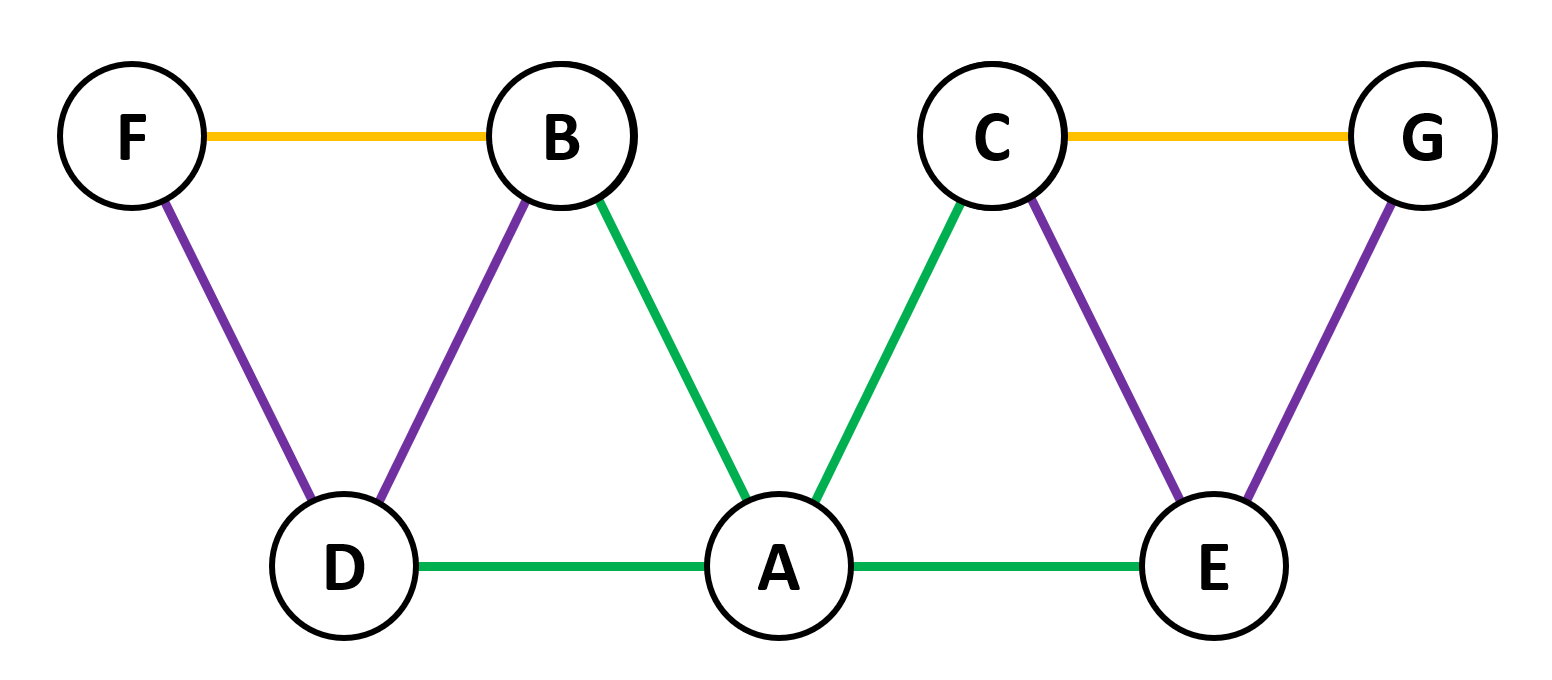
\includegraphics[width=0.7\textwidth]{P1p1.png}
\caption{Graph for BFS traversal.}
\label{fig:graphsol}
\end{figure}

\noindent Constructing the BFS forest:
\begin{itemize}
    \item \(a \rightarrow b\)
    \item \(a \rightarrow c\)
    \item \(a \rightarrow d\)
    \item \(a \rightarrow e\)
    \item \(b \rightarrow f\)
    \item \(c \rightarrow g\)
\end{itemize}
A Graphical representation is in Figure \ref{fig:bfsforest}.

\begin{figure}[h]
\centering
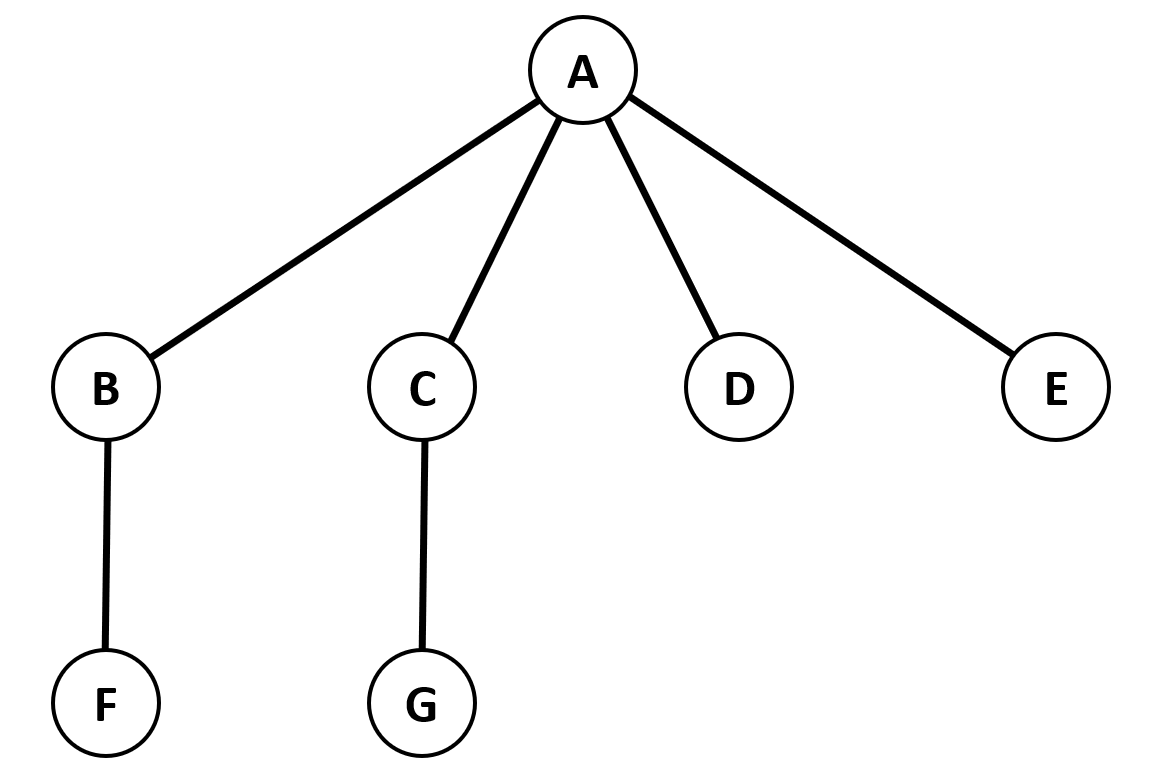
\includegraphics[width=0.7\textwidth]{P1p2.png}
\caption{BFS Forest Diagram(Tree)}
\label{fig:bfsforest}
\end{figure}
\newpage
\noindent Tree edges (as determined by BFS traversal):

\begin{itemize}
    \item \(a \rightarrow b\)
    \item \(a \rightarrow c\)
    \item \(a \rightarrow d\)
    \item \(a \rightarrow e\)
    \item \(b \rightarrow f\)
    \item \(c \rightarrow g\)
\end{itemize}
\noindent Now, for the cross edges, we look at the remaining connections:
\begin{itemize}
    \item \(b \rightarrow d\): Neither `b' nor `d' is an ancestor of the other in the BFS tree.
    \item \(c \rightarrow e\): Neither `c' nor `e' is an ancestor of the other in the BFS tree.
    \item \(e \rightarrow g\): Neither `e' nor `g' is an ancestor of the other in the BFS tree.
    \item \(f \rightarrow d\): Neither `f' nor `d' is an ancestor of the other in the BFS tree.
\end{itemize}
\noindent In summary:

\begin{itemize}
    \item Tree Edges: \([a \rightarrow b]\), \([a \rightarrow c]\), \([a \rightarrow d]\), \([a \rightarrow e]\), \([b \rightarrow f]\), \([c \rightarrow g]\)
    \item Cross Edges: \([b \rightarrow d]\), \([c \rightarrow e]\), \([e \rightarrow g]\), \([f \rightarrow d]\)
\end{itemize}

No edge in this BFS traversal is a back or forward edge.
\newpage
\section*{Problem \#2}

(25 points) Apply the DFS-based algorithm to solve the topological sorting problem for the following directed graph below:

\begin{figure}[h]
\centering
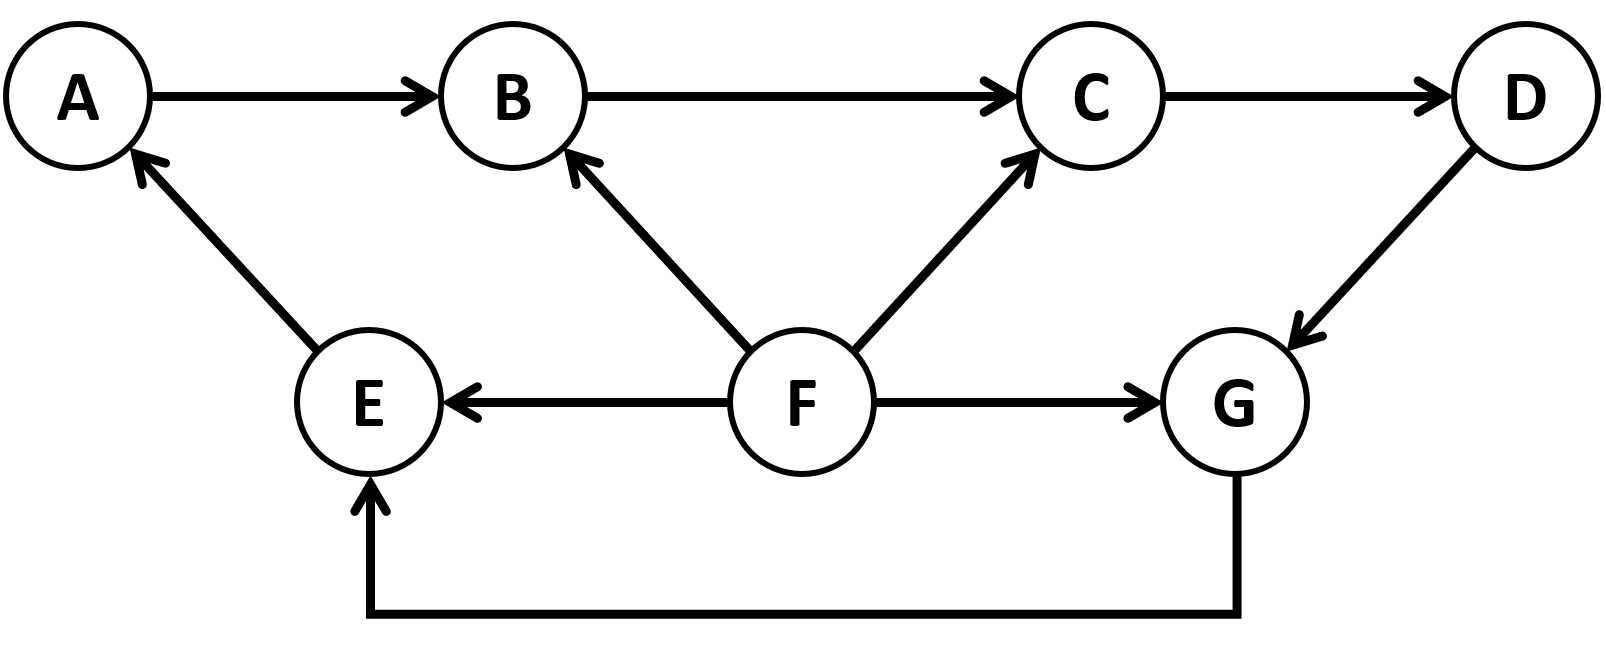
\includegraphics[width=0.7\textwidth]{P2.png}
\caption{Directed Graph depicting relationships between vertices A to G.}
\label{fig:Prob2}
\end{figure}

\noindent Start the traversal at vertex `a` and resolve ties by alphabetical ordering. You are required to:

\begin{enumerate}
  \item[(i)] (7 points) Show the traversal stack
  \item[(ii)] (7 points) Draw the DFS forest including tree edges and other types of edges
  \item[(iii)] (4 points) List the number of tree edges, back edges, forward edges and cross edges in the forest
  \item[(iv)] (3 points) Give the order of vertices visited (both push-in \& pop-off order)
  \item[(v)] (4 points) Does a topological sorting solution exist for this graph? If yes, write the topological sorting order; if not, explain why?
\end{enumerate}

\subsection*{Solution}
\subsection*{Traversal Stack:}

\begin{enumerate}
    \item \(A\) is pushed. Stack: \([A]\)
    \item \(B\) is pushed. Stack: \([A, B]\)
    \item \(C\) is pushed. Stack: \([A, B, C]\)
    \item \(D\) is pushed. Stack: \([A, B, C, D]\)
    \item \(G\) is pushed. Stack: \([A, B, C, D, G]\)
    \item \(E\) is pushed. Stack: \([A, B, C, D, G, E]\)
    \item \(E\) is popped. Stack: \([A, B, C, D, G]\)
    \item \(G\) is popped. Stack: \([A, B, C, D]\)
    \item \(D\) is popped. Stack: \([A, B, C]\)
    \item \(C\) is popped. Stack: \([A, B]\)
    \item \(B\) is popped. Stack: \([A]\)
    \item \(F\) is pushed. Stack: \([A, F]\)
    \item \(F\) is popped. Stack: \([A]\)
    \item \(A\) is popped. Stack: \([]\)
\end{enumerate}

\subsection*{DFS Forest:}
\begin{figure}[h]
\centering
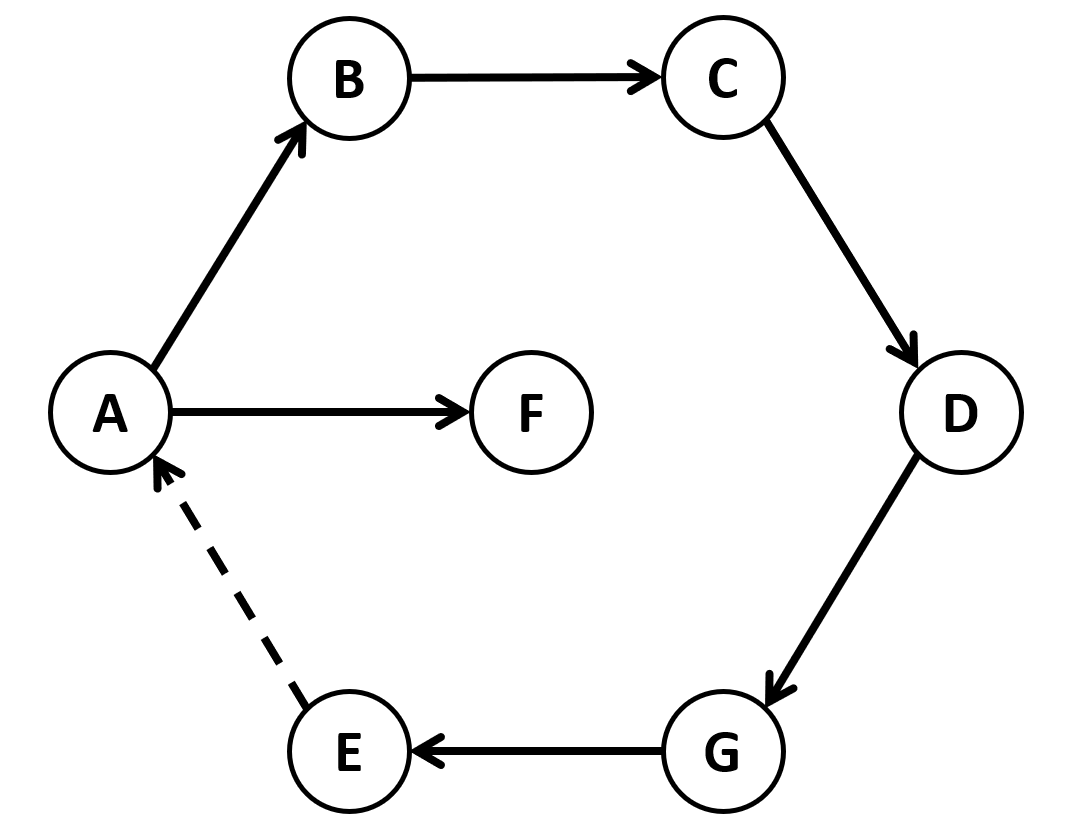
\includegraphics[width=0.7\textwidth]{P2p1.png}
\caption{DFS Forest with Tree and Back Edges}
\label{fig:dfsforest}
\end{figure}

\subsection*{Number of Edges:}
\begin{itemize}
    \item Tree Edges: 6 \([A \rightarrow B]\), \([B \rightarrow C]\), \([C \rightarrow D]\), \([D \rightarrow G]\), \([G \rightarrow E]\), \([A \rightarrow F]\)
    \item Back Edges: 1 \([E \rightarrow A]\)
    \item Forward Edges: 0
    \item Cross Edges: 4 \([F \rightarrow E]\), \([F \rightarrow B]\), \([F \rightarrow C]\), \([F \rightarrow G]\)
\end{itemize}

\subsection*{Order of Vertices Visited:}
Push-In Order: \(A, B, C, D, G, E, F\)
\newline
Pop-Off Order: \(E, G, D, C, B, F, A\)

\subsection*{Topological Sorting:}
A directed graph has a topological sort if and only if it has no directed cycles. The presence of a back edge (\(E \rightarrow A\)) indicates a directed cycle. 
\newline\newline
Thus, a topological sorting solution does \textbf{not} exist for this graph.
\newpage
\section*{Problem \#3}

(25 points) Apply the Source-Removal algorithm to the graph in the figure to solve the topological sorting problem for the directional graph below.

\begin{figure}[h]
\centering
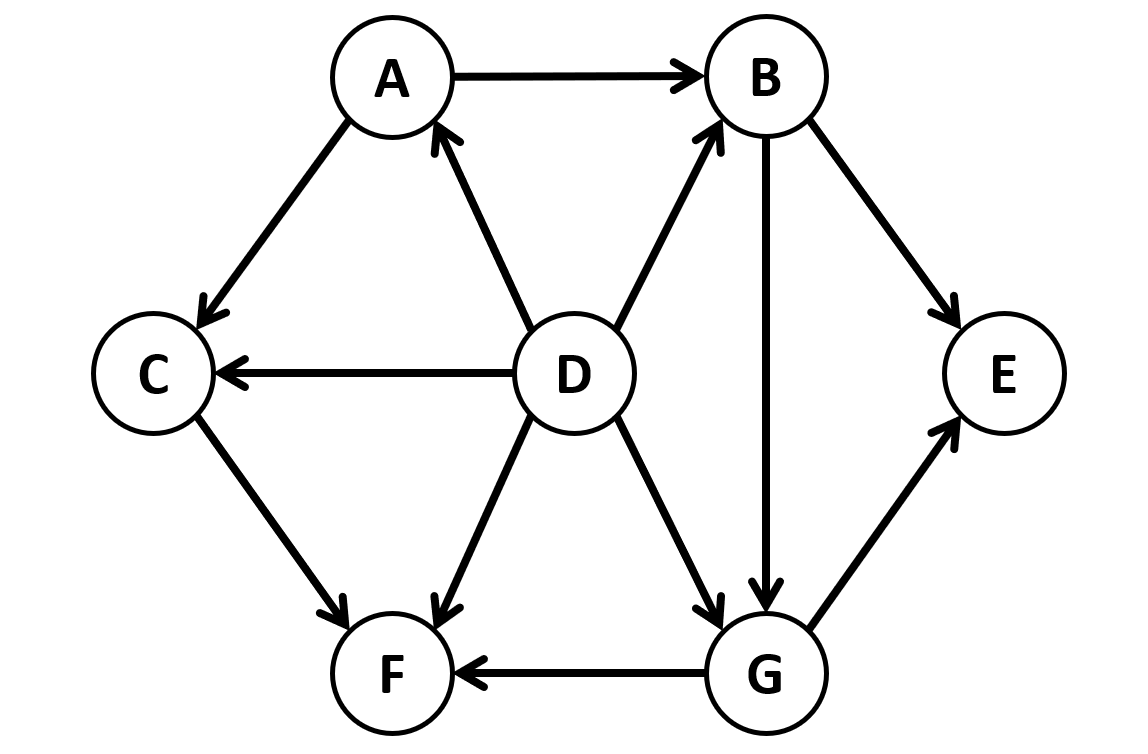
\includegraphics[width=0.7\linewidth]{P3.png}
\caption{Directional Graph}
\end{figure}

\noindent \textbf{Requirements:}
\begin{itemize}
    \item Redraw the graph after each source is eliminated.
    \item Does a topological sorting solution exist for this graph? If yes, write the topological sorting order; if not, explain why?
\end{itemize}

\subsection*{Solution}
Using the Source Removal algorithm, we proceed to remove vertices that have no incoming edges. The process is illustrated as follows:

\begin{enumerate}
    \item Remove \( D \). This vertex is removed because it has no incoming edges.
    \item Remove \( A \). After removing \( D \), \( A \) has no incoming edges.
    \item Remove \( B \). Following the removal of \( D \) and \( A \), \( B \) becomes a source vertex.
    \item Remove \( C \). \( C \) also has no incoming edges.
    \item Remove \( G \). With previous removals, \( G \) becomes a source vertex.
    \item Remove \( E \). \( E \) is next since it now has no incoming edges.
    \item Remove \( F \). Lastly, \( F \) is removed as it has no incoming edges.
\end{enumerate}

\section*{Redrawn Graphs}
The graph after each step of the source removal algorithm is illustrated below.

\begin{figure}[h]
\centering
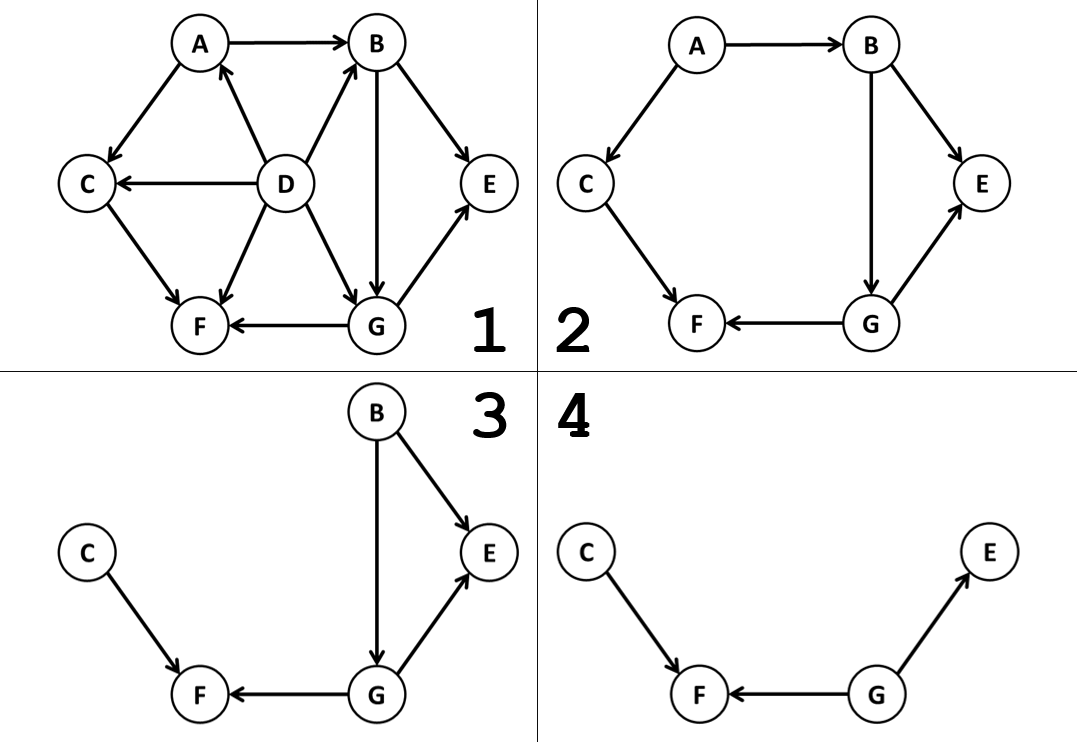
\includegraphics[width=0.55\linewidth]{P3p1.png}
\caption{Graph after removing \( D, A \) and \( B \)}
\end{figure}

\begin{figure}[h]
\centering
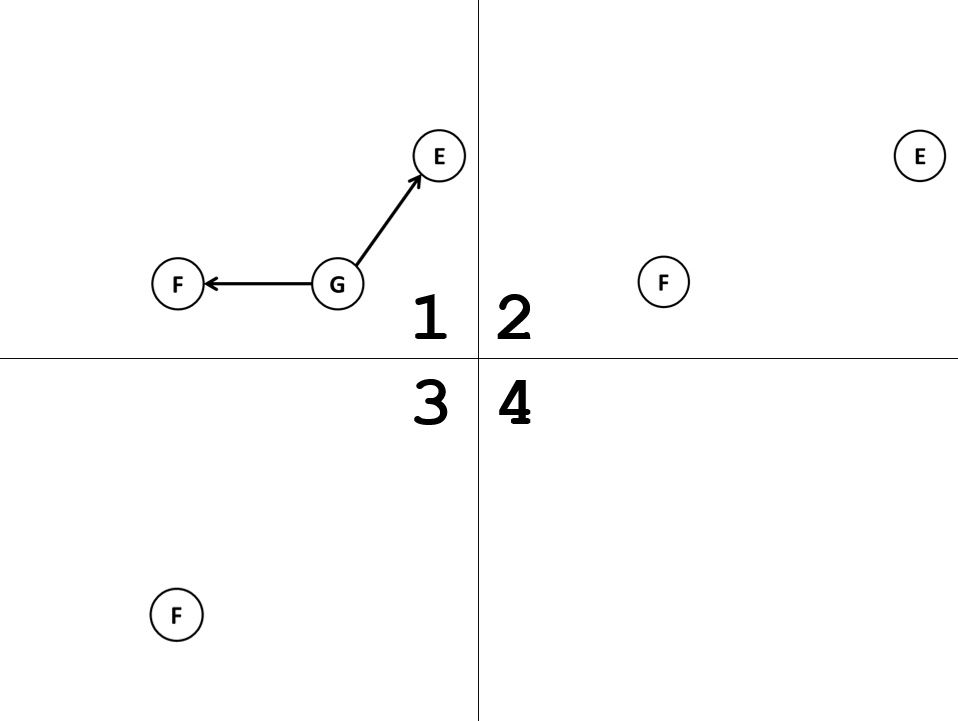
\includegraphics[width=0.55\linewidth]{P3p2.png}
\caption{Graph after removing remaining vertices}
\end{figure}

\subsubsection*{Topological Ordering}
After following the source removal method, all nodes are successfully removed indicating that the graph has a valid topological ordering: \( D, A, B, C, G, E, F \).

\newpage

\section*{Problem \#4}
Find the \( n \)-th smallest element in the following list using the QuickSelect algorithm. For this example, let \( n=2 \). \\
Actual List: \([77, 19, 11, 31, -51, 42, -4]\)

\subsection*{Solution for Finding the 2nd Smallest Element (\( n=2 \))}
\begin{enumerate}
\item \textbf{1st Pivot (77)}: 
    \begin{align*}
        \text{List:} & \quad [77, 19, 11, 31, -51, 42, -4] \\
        \text{Position:} & \quad 7\text{th smallest}
    \end{align*}

\item \textbf{2nd Pivot (19)}: 
    \begin{align*}
        \text{List:} & \quad [77, 31, 42, 19, 11, -51, -4] \\
        \text{Position:} & \quad 4\text{th smallest}
    \end{align*}

\item \textbf{3rd Pivot (11)}: 
    \begin{align*}
        \text{List:} & \quad [77, 31, 42, 19, 11, -51, -4] \\
        \text{Position:} & \quad 3\text{rd smallest}
    \end{align*}

\item \textbf{4th Pivot (-51)}: 
    \begin{align*}
        \text{List:} & \quad [77, 31, 42, 19, 11, -4, -51] \\
        \text{Position:} & \quad 1\text{st smallest}
    \end{align*}

\item \textbf{5th Pivot (-4)}: 
    \begin{align*}
        \text{List:} & \quad [77, 31, 42, 19, 11, -4, -51] \\
        \text{Position:} & \quad 2\text{nd smallest}
    \end{align*}

\item \textbf{Result}: The 2\textsuperscript{nd} smallest element is \( -4 \).

\end{enumerate}
\end{document}
